\documentclass[a4paper,11pt,dvipdfmx]{jsarticle}

\usepackage{bm}
\usepackage[dvipdfmx]{graphicx}
\usepackage[dvipdfmx]{color}
\usepackage{ascmac}
\usepackage{siunitx}
\usepackage{otf}
\pagestyle{plain}
%\usepackage[subrefformat=parens]{subcaption}
\usepackage{float}
\usepackage[dvipdfmx]{hyperref}
\usepackage{pxjahyper}
\usepackage{here}
\usepackage{titlesec}
\titleformat*{\section}{\LARGE\bfseries}
\titleformat*{\subsection}{\normalsize\bfseries}
\usepackage{url}
\usepackage[table,xcdraw]{xcolor}
\hypersetup{% hyperrefオプションリスト
setpagesize=false,
 bookmarksnumbered=true,%
 bookmarksopen=true,%
 colorlinks=true,%
 linkcolor=blue,
 citecolor=blue,
}


\begin{document}
\newpage
\section{\LARGE{議論と考察(担当:木村)}}

\subsection{目的}
本章ではこれまでの解析から得られた微分散乱断面積の評価を行う。炭素においては核力による微分散乱断面積から原子核半径の推定を行う。また2つの検出を用いた2チャンネル同時計測により、p-p散乱の観測を試みる。

\subsection{微分散乱断面積の評価}
\subsubsection{文献値との比較}
本実験では金とポリエチレン(水素と炭素)をターゲットとして用い、それらの微分散乱断面積を導出した。微分散乱断面積の文献値はRutherfordの公式より
\begin{equation}
    \frac{d\sigma}{d\Omega} = \left(\frac{Z_1Z_2e^2}{16\pi\epsilon_0E}\right)^2\frac{1}{\sin^4{\frac{\theta}{2}}}
    \label{siki1}
\end{equation}
で表される。この文献値はクーロン力のみを考慮しているため、金に対して考察を行う。その際に、測定値に fit 線を引くことにより文献値との比較を行う。具体的には
\begin{equation}
    (fit線) = [p_0] \times \left(\frac{Z_1Z_2e^2}{16\pi\epsilon_0E}\right)^2\frac{1}{\sin^4{\frac{\theta}{2}}}
    \label{crosssection}
\end{equation}
という式をfittingに用いる。この式は式(\ref{siki1}) に定数 p0 をかけており、p0をパラメーターとして動かし、測定値に最小二乗法を用いてfitさせる。この線を引くことで、fit 線に測定値が乗っているかどうかを評価する。また p0 が1に近いほど文献値と一致していると言えるので、その点も評価対象とする。
\subsubsection{金の微分散乱断面積}
まずは核力の影響しないターゲットである金の微分散乱断面積から考察していく。図\ref{aucs}に微分散乱断面積の測定値、文献値、fit線を示す。パラメータ p0 はほとんど 1 に近く、測定点は fit 線によく乗っている。ただし、110$^{\circ}$の点については除外している。その理由については次節で記述する。また100$^\circ$と120$^\circ$の点についてもノイズが少しはいっていたが、110$^\circ$の点に比べ、ノイズが小さかったので残した。
\begin{figure}[H]
\centering
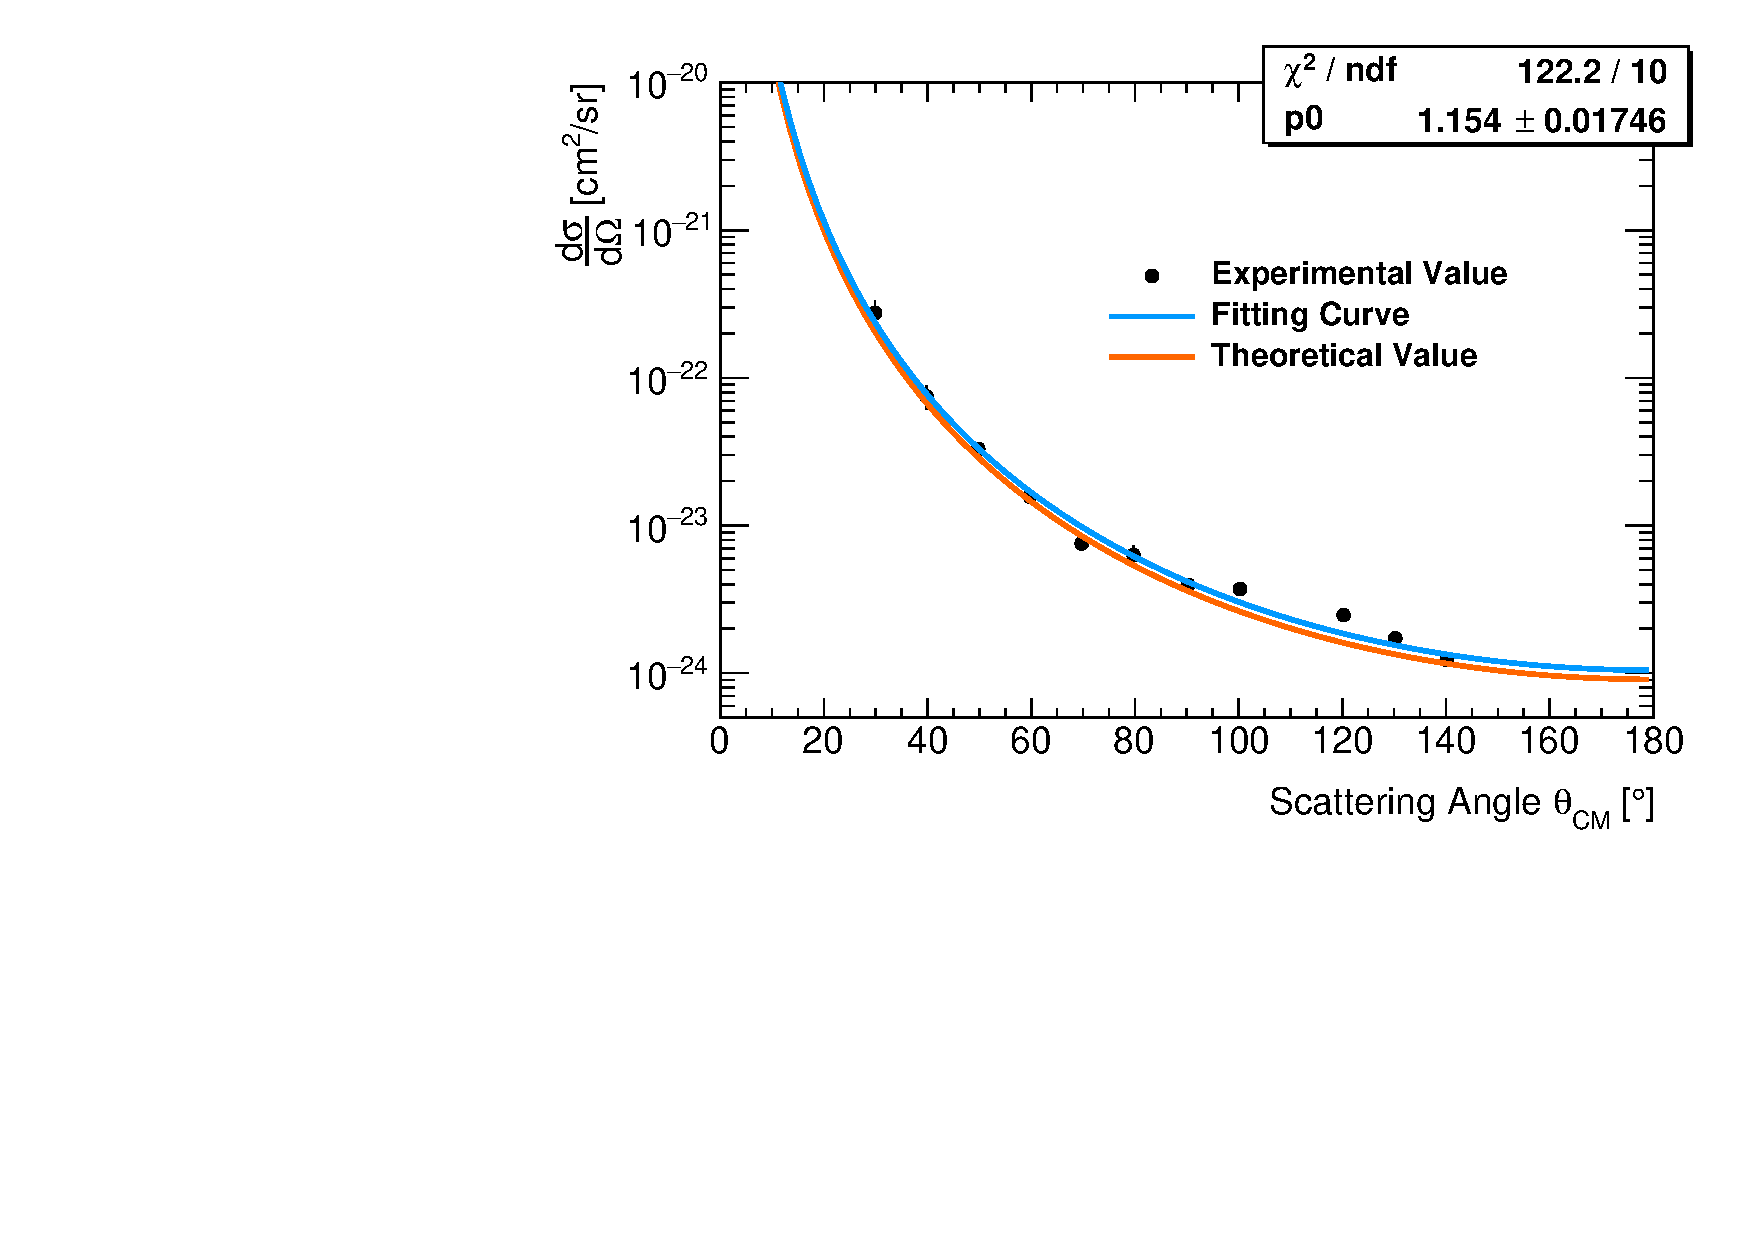
\includegraphics[width=100mm]{picture/jan/Au_CM.pdf}
\caption{金の微分散乱断面積}
\label{aucs}
\end{figure}

図\ref{sp110}は測定角度110$^\circ$のスペクトルである。ノイズがはいっており、散乱陽子数を精度良く求められない。測定角度70$^\circ$のスペクトル(図\ref{sp70})と比較するとノイズがはいってきているのは明らかである。このノイズはターゲットにより散乱されたものではなく、ターゲットホルダーなどの別の物質によって散乱された陽子が観測されているものと考えられる。微分散乱断面積は以下の式で算出する。\\\\
\begin{equation}
    \frac{d\sigma}{d\Omega} = \frac{N\times e \times A}{d\Omega \times I \times T \times d \times t \times N_A}
    \label{expcross}
\end{equation}\\
微分散乱断面積は散乱陽子数に依り、110$^\circ$の点を含めると正確な算出が困難になるため、今回は除外した。\\\\
\begin{figure}[H]
\begin{minipage}{0.5\hsize}
\begin{center}
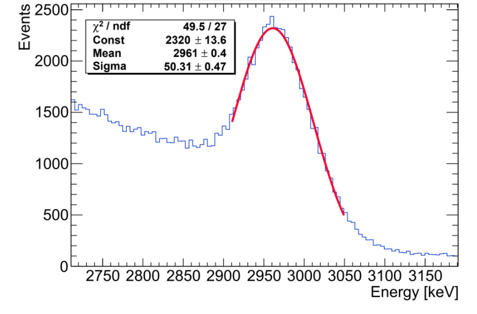
\includegraphics[width=70mm]{picture/jan/110hist.png}
\end{center}
\caption{110$^\circ$におけるスペクトル}
\label{sp110}
\end{minipage}
\begin{minipage}{0.5\hsize}
\begin{center}
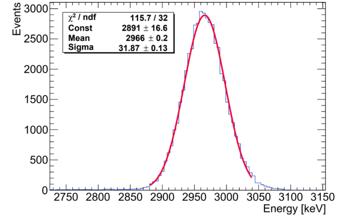
\includegraphics[width=70mm]{picture/jan/70hist.png}
\end{center}
\caption{70$^\circ$におけるスペクトル}
\label{sp70}
\end{minipage}
\end{figure}
\subsubsection{炭素の微分散乱断面積}\label{C1}
炭素の微分散乱断面積の導出にはポリエチレンをターゲットとして用いている。また炭素の場合は陽子が原子核に達することがあるので、クーロン力だけでなく核力による散乱も考慮する必要がある。この時の文献値は\ref{NF}より、
\begin{equation}
    \frac{d\sigma}{d\Omega} = \left(\frac{Z_1Z_2e^2}{16\pi\epsilon_0E}\right)^2\frac{1}{\sin^4{\frac{\theta}{2}}} + \frac{R^2}{4}
\end{equation}
となる。したがって、炭素の微分散乱断面積のfittingはこの式を用いて行う。この核力による微分散乱断面積を用いて原子核半径の推定も行う。図\ref{tanso1}に炭素の微分散乱断面積の測定値、文献値、fit線を書いている。理論値とのズレが大きく、ポリエチレンの炭化によって厚さ・密度が変化している可能性が考えられる。次節において炭化による厚さと密度の変化量を見積もる。
\begin{figure}[H]
\centering
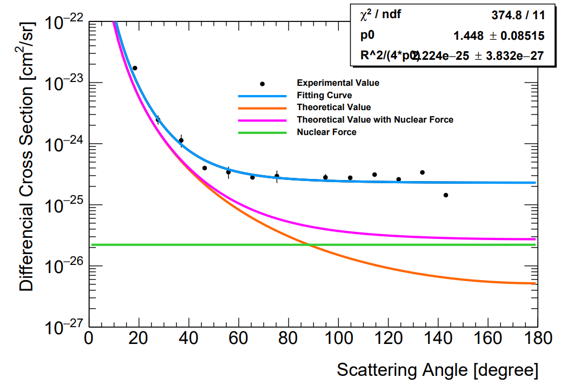
\includegraphics[width=100mm]{picture/jan/C1.png}
\caption{炭素の微分散乱断面積}
\label{tanso1}
\end{figure}
\subsubsection{炭化の考慮}
先行研究\cite{2019}よりポリエチレンは無酸素状態で熱することで炭化し、炭化した場合の密度はしない場合の約2倍であることがわかっていた。ポリエチレンが炭化したことにより(\ref{expcross})式の $d \times t$ の値が変化し、微分散乱断面積にズレが生じていので厚さ・密度の再測定を行った。$\alpha$線のエネルギーを、ターゲットに当てた場合とターゲットなしの場合で比較し、Bethe-Blochの式を用いてエネルギー損失から$d \times t$の推定を行った。その結果、以下の値が得られた。
\begin{equation}
d\times t = (1.61\pm 0.02)\times 10^{-3} \:\: \text{(g/cm$^2$)}
\end{equation}
この値は炭化を考慮する前と比較すると2倍程度ずれていることが分かる。図\ref{tanka1}に炭化を考慮した炭素の微分散乱断面積の測定値、文献値、fit線を示す。
\begin{figure}[H]
\centering
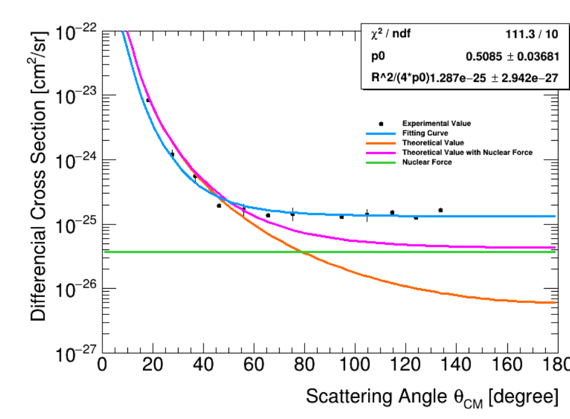
\includegraphics[width=110mm]{picture/jan/C2.png}
\caption{炭素の微分散乱断面積(炭化を考慮)}
\label{tanka1}
\end{figure}

\label{C2}
炭素の原子核半径の推定には炭化を考慮した図\ref{tanka1}を用いる。グラフより
\begin{equation}
\frac{R^2}{4} = (6.54\pm 1.92)\times 10^{-26} \text{cm}^2
\end{equation}
これより
\begin{equation}
R = 5.12\pm 0.75\ \text{fm}
\end{equation}
この時、$R$は原子核半径と陽子半径の和であるから、陽子半径 0.87 fm を引いて
\begin{equation}
r_c = 4.25\pm 0.75\ \text{fm}
\label{tankasiki}
\end{equation}

\newpage
\subsubsection{核力の補正と考察}
\ref{C1}、\ref{C2}節で行った解析は核力による散乱断面積を古典的に導出したものを使用していた。ここで\ref{kakuhosei}節で述べたように量子論を考慮した散乱断面積を導入する。炭素の原子核半径は表\ref{table:gensi}より、$r_c=2.97 $ fmであることを用いて補正を行った。[図\ref{c_cs_hosei}]
\begin{figure}[H]
    \centering
        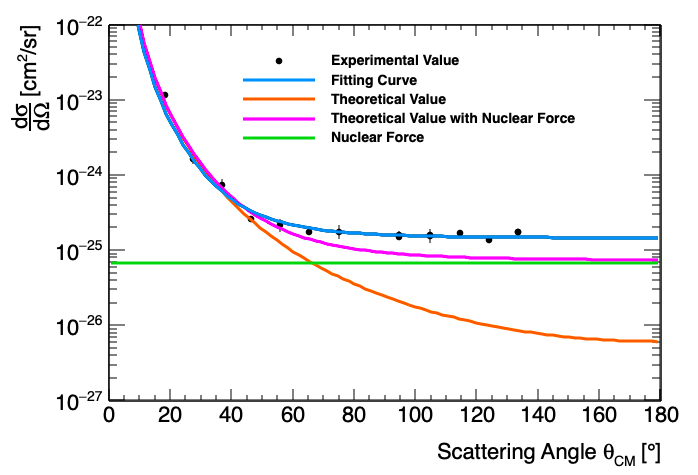
\includegraphics[width=110mm]{picture/jan/C5.png}
    \caption{炭素の微分散乱断面積(核力の補正あり)}
    \label{c_cs_hosei}
\end{figure}
図\ref{tanka1}と比較してfitting関数がより実験値に近づいていることが分かる。ここで、fittingパラメータp0 $= 0.76 \pm 0.04$であった。またfittingによって得られた核力による微分散乱断面積は、
\begin{equation}
    \frac{d\sigma}{d\Omega} = \left( 1.081 \pm 0.109 \right) \times 10^{-25} \:cm^2/sr
\end{equation}
であった。\ref{kakuhosei}節より$\frac{d\sigma}{d\Omega}=R^2$と近似できるのでこれを用いて原子核半径を求めると
\begin{equation}
    R = 3.29 \pm 0.05 \: fm
\end{equation}
と算出され、\ref{tankasiki}式より理論値2.97 fmに近づいたものの、誤差の範囲内には収まらなかった。これは\ref{kakuhosei}節における近似によるものであると考えられる。まず、S波のみが散乱断面積に寄与するのは$\lambda \gg R$の条件下である。今回入射波長は$\lambda=16.52\:$fmであるため、$\lambda \gg R$とは言い難い。そのため正確な断面積の導出には、$l\geq1$における散乱振幅を考えなければならない。また$\frac{d\sigma}{d\Omega}=R^2$の関係式も同様の条件のもとでの近似式であるので、厳密には異なる。

\newpage
\subsubsection{水素の微分散乱断面積}
続いて、水素の散乱断面積を求めた。図\ref{expmott}に水素を標的とした際の散乱断面積とfitting曲線、そして理論値を示す。
\begin{figure}[H]
\centering
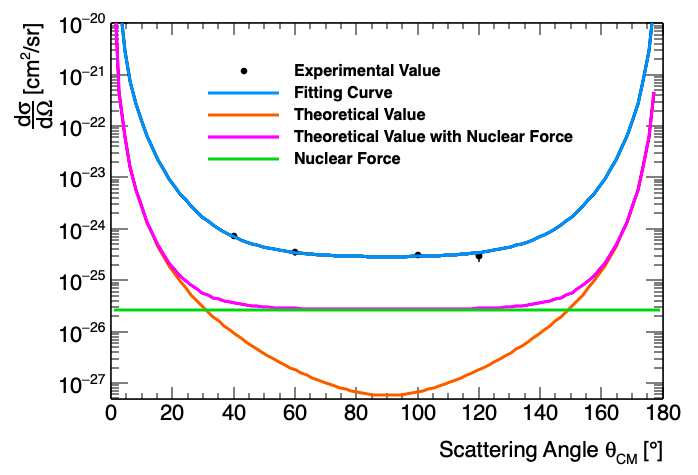
\includegraphics[width=100mm]{picture/jan/H2.png}
\caption{水素の微分散乱断面積}
\label{expmott}
\end{figure}
図\ref{expmott}より、散乱断面積の実測値は理論値と比較してオーダー1つ大きいような結果となった(fittingパラメータ p0$=47.28$)。原因として考えられるのは、Mottの散乱公式(\ref{eq:Mott})に対して、核力による散乱が本研究で考慮している理論値より多くはたらいていることが挙げられる。\ref{kakuhosei}の核力は異種粒子間の散乱を前提としていること、反跳水素原子核についても散乱断面積を導出していないことが原因として考えられる。それらの考慮を行うことでMott散乱のより正確な測定や、水素原子核(陽子)の半径を求めることができると考えた。


\newpage
\subsection{p-p散乱}
\subsubsection{p-p散乱の観測}
\ref{opening}節よりp-p散乱の opening angle は非相対論では90$^{\circ}$であるから、その観測においてp-p散乱が見られるかどうかを考えていく。角度のとり方を図\ref{kakudo}に示す。図\ref{4050}は40$^{\circ}$と50$^{\circ}$における2つの検出器でのエネルギーの相関を表した二次元ヒストグラムである。図\ref{fig:scaene}と図\ref{fig:recoil}よりそれぞれのエネルギーを対応させると、この二次元ヒストグラムからコインシデンスが上手くとれていることが分かるので、40$^{\circ}$と50$^{\circ}$の同時計測ではp-p散乱が見ることができたと結論づけた。
\begin{figure}[H]
    \begin{tabular}{cc}
      \begin{minipage}[t]{0.45\hsize}
        \centering
        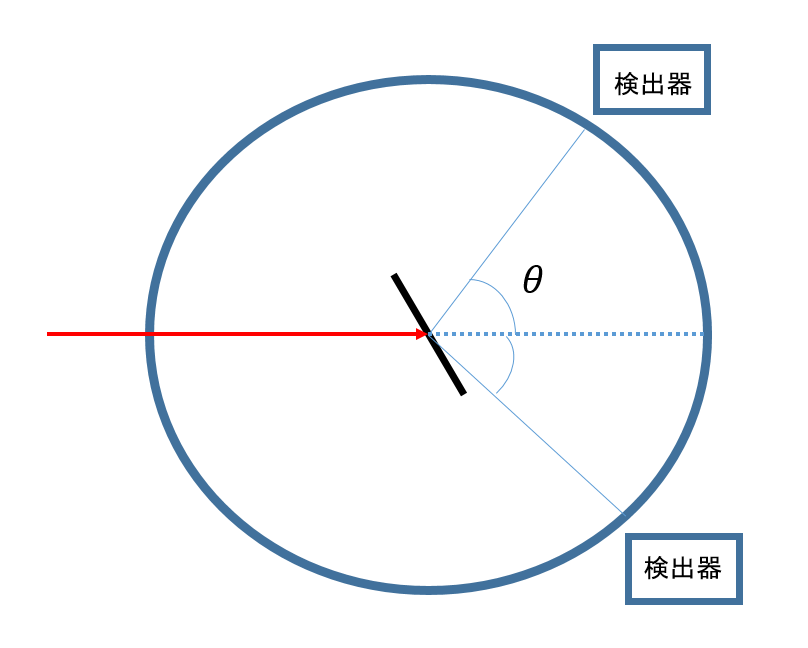
\includegraphics[width=70mm]{picture/jan/kakudo.png}
        \caption{角度のとり方}
        \label{kakudo}
      \end{minipage} &
      \begin{minipage}[t]{0.45\hsize}
        \centering
        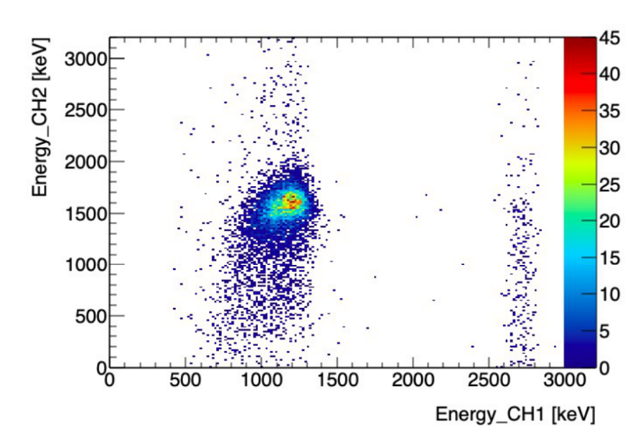
\includegraphics[width=70mm]{picture/jan/4050.png}
        \caption{40$^{\circ}$と50$^{\circ}$の同時計測(CH1が50$^\circ$、CH2が40$^\circ$)}
        \label{4050}
      \end{minipage}
    \end{tabular}
\end{figure}
また図\ref{hist3060}、図\ref{hist2070}はそれぞれ30$^{\circ}$と60$^{\circ}$、20$^{\circ}$と70$^{\circ}$の2つの検出器でのエネルギーの相関を表した二次元ヒストグラムである。表\ref{rironchi}より、予想されるエネルギー帯においてコインシデンスがとれておらず、p-p散乱を観測できていないということが分かる。60$^{\circ}$や70$^{\circ}$のような大角度はp-p散乱が見られなかった。また理論値と異なるだけでなく、観測されたイベントレートも非常に小さかったため、これらの信号は偶発的なものである可能性が高い。

\vspace*{7mm}

\begin{table}[h]
   \caption{p-p散乱におけるエネルギー理論値(標的中でのエネルギー損失は考慮していない)}
   \centering
 \begin{tabular}{cc} \hline
  散乱角度のペア [$^\circ$] & エネルギー理論値 [MeV] \\ \hline \hline
  
  \begin{tabular}{c}
    40 - 50  \\
    30 - 60 \\
    20 - 70 \\
   \end{tabular} &
   
  \begin{tabular}{c}
    1.76 - 1.24 \\
    2.25 - 0.75 \\
    2.65 - 0.35 \\
  \end{tabular} 
   \\ \hline
   \end{tabular}
   \label{rironchi}
\end{table}

\begin{figure}[H]
    \begin{tabular}{cc}
      \begin{minipage}[t]{0.45\hsize}
        \centering
        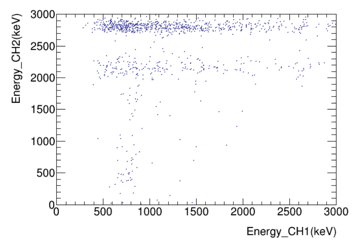
\includegraphics[width=70mm]{picture/jan/3060.png}
        \caption{30$^{\circ}$と60$^{\circ}$の同時計測(CH1が60$^\circ$、CH2が30$^\circ$)}
        \label{hist3060}
      \end{minipage} &
      \begin{minipage}[t]{0.45\hsize}
        \centering
        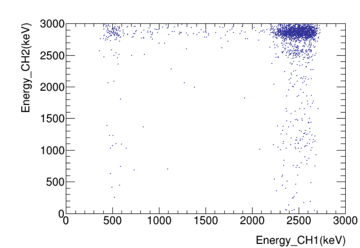
\includegraphics[width=70mm]{picture/jan/2070.png}
        \caption{20$^{\circ}$と70$^{\circ}$の同時計測(CH1が70$^\circ$、CH2が20$^\circ$)}
        \label{hist2070}
      \end{minipage}
    \end{tabular}
\end{figure}


大角度においてp-p散乱が見られなかった原因として、60,70$^\circ$における信号がディスクリミネーターのthresholdよりも小さく、パルスが出力されていなかった可能性が挙げられる。そこでパルスジェネレーターを用いて、PHADCの値を電圧に換算することでthreshold電圧と比較した。図\ref{PHADC_V}はPHADCの値と電圧の換算直線、60$^{\circ}$と70$^{\circ}$におけるPHADCの理論値、ディスクリミネーターのthreshold電圧を示したグラフである。thresholdはおよそ100mVであり、グラフより60$^{\circ}$および70$^{\circ}$のPHADCの値は電圧に換算するとthresholdよりも低いことが分かる。したがって、このことが原因でp-p散乱が見られなかったと言える。\\
 20-70$^\circ$、30-60$^\circ$の計測においてp-p散乱を観測するにはthreshold電圧を下げる必要がある。ノイズ落としを行う、より低エネルギーでも分解能のある検出器を利用する、などで改善が見込まれる。
 \begin{figure}[H]
 \centering
 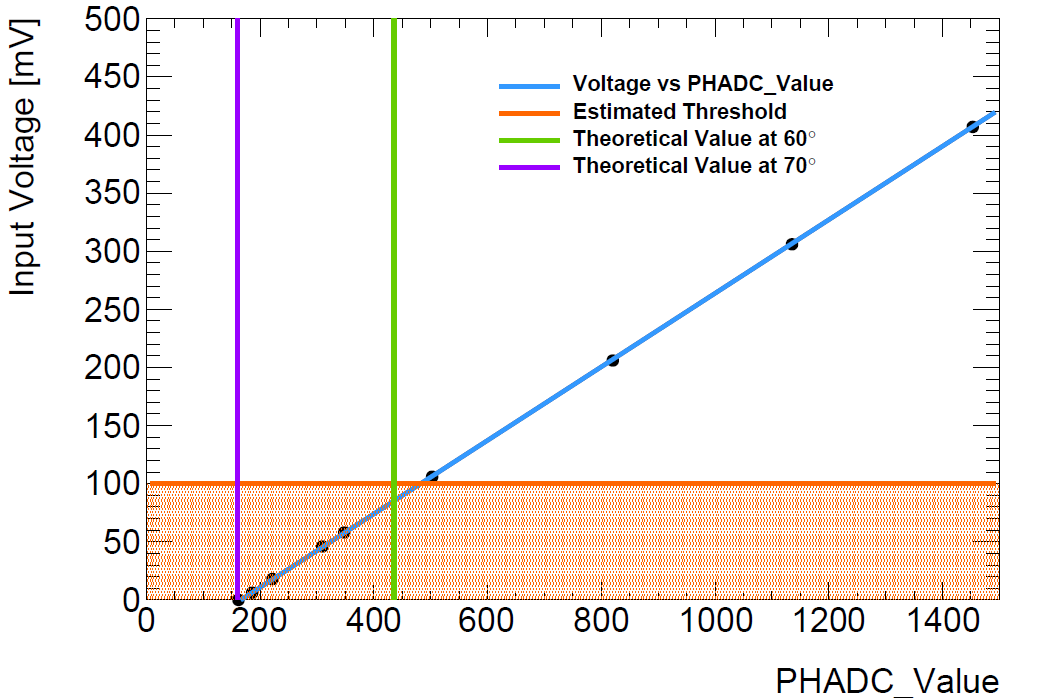
\includegraphics[width=95mm]{picture/jan/parujene.png}
 \caption{PHADCの値と電圧の換算直線}
 \label{PHADC_V}
 \end{figure}
 \begin{figure}[H]
 \centering
 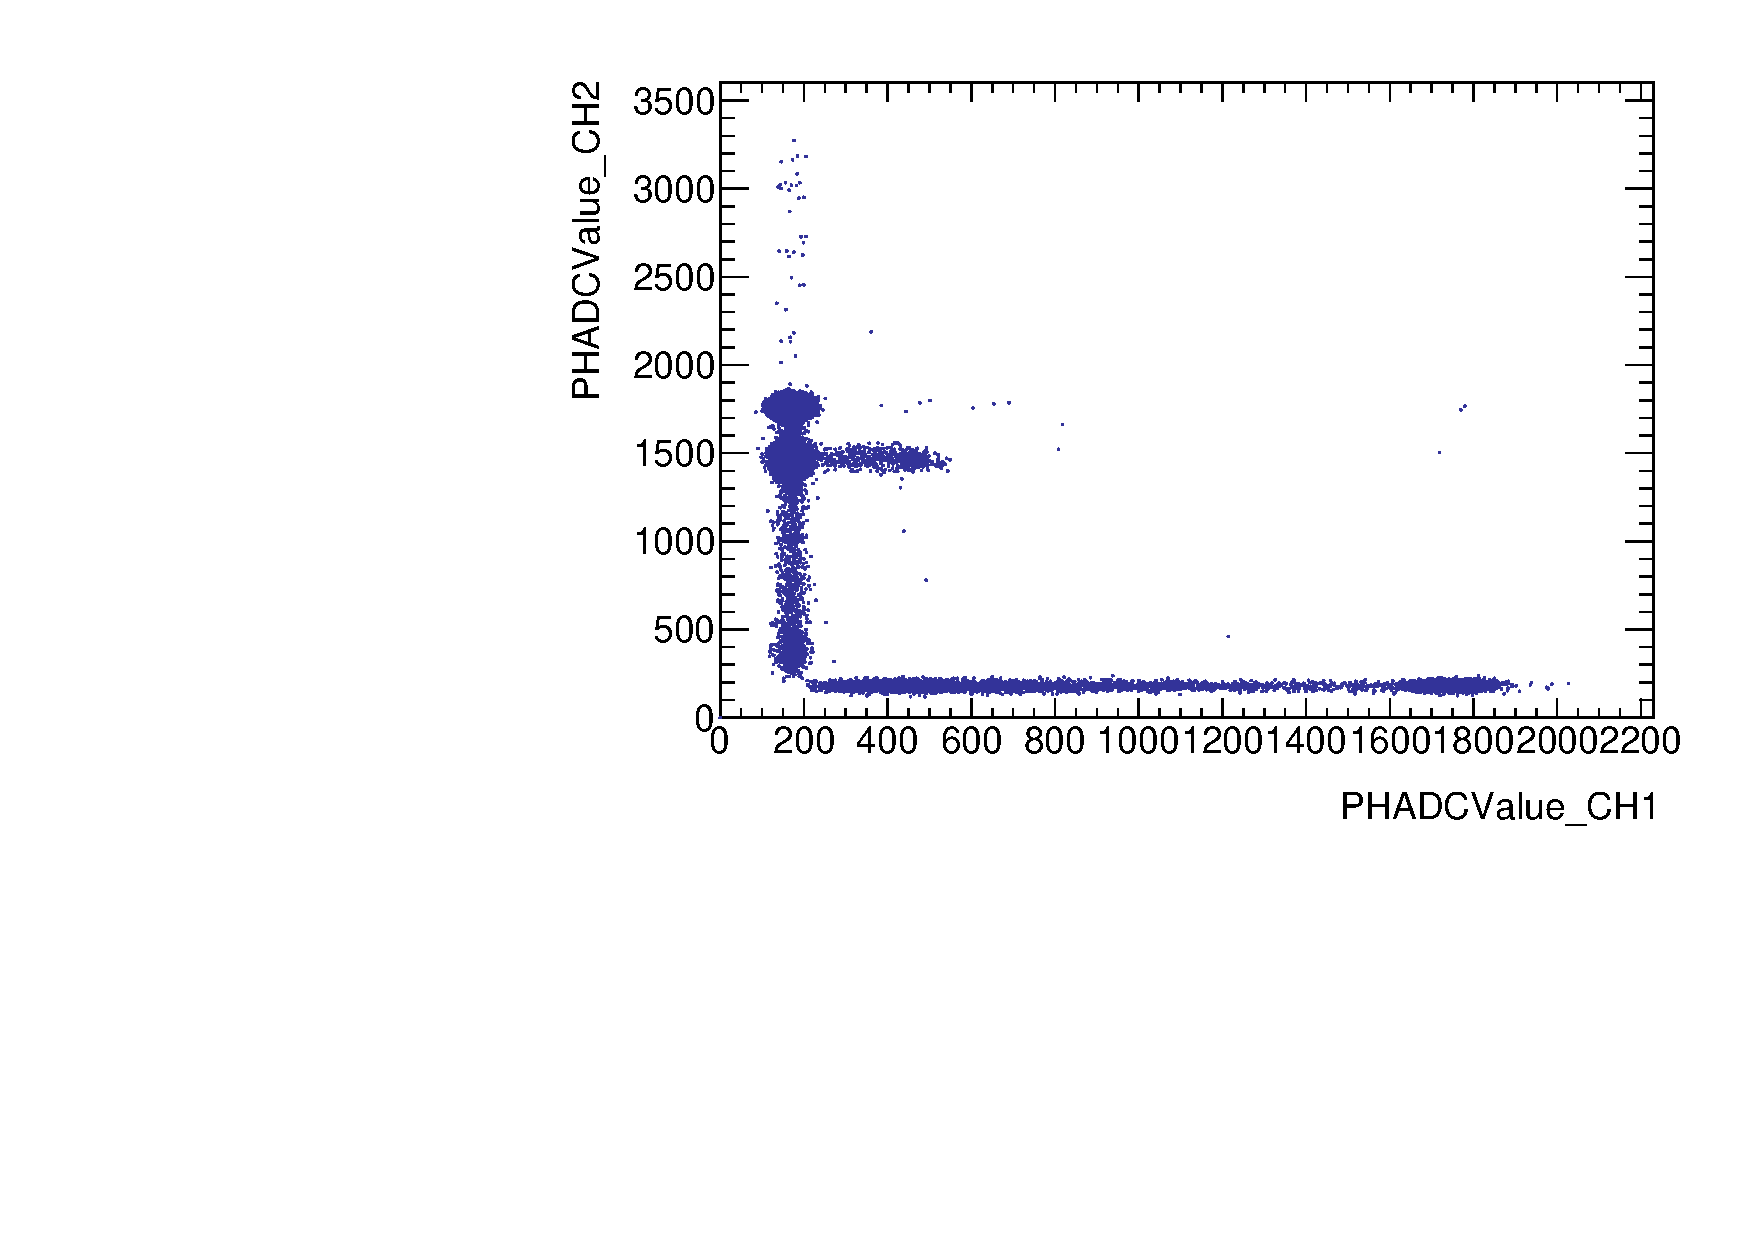
\includegraphics[width=90mm]{picture/jan/Ratio_09run6.pdf}
 \caption{30$^\circ$と60$^\circ$の同時計測(ANY1)}
 \label{any1}
 \end{figure}
 図\ref{any1}は30$^\circ$と60$^\circ$をコインシデンスモジュールのANY1機能を用いて観測を行ったものである。ANY1機能については\ref{logic}節において説明している。ANY1での観測において理論値の近傍に点の集合が見られた。これはコインシデンスがとれていなかったという仮説と矛盾せず、threshold電圧より小さい信号が出ていたという仮説を裏付ける。
 
 \subsubsection{その他の候補}
大角度になるほど散乱陽子と反跳養子にエネルギー、すなわち速度の差が生じ、検出器に届くまでの時間がずれてコインシデンスが上手くとれないという原因も考えうる。
散乱してから検出器に届くまでの時間は30$^{\circ}$では5.70 ns、60$^{\circ}$では3.32 nsであるから、その差は約2.38 nsである。
%散乱してから検出器に届くまでの時間は、20$^{\circ}$では2.97 ns,60$^{\circ}$で8.17  nsであるから、その差は約5 nsである。
ディスクリミネーターの最小出力幅は10nsであり、今研究での設定値はおよそ100nsであるからこの可能性は考えにくい。20-70$^\circ$に関してもその差は約2.5 nsという結果であり、コインシデンスをとるには十分な時間差であると結論づけた。

 \subsection{まとめ}
本実験では原子核散乱による陽子のエネルギースペクトル、角度、散乱陽子数などを解析し、微分散乱断面積の評価、炭素の原子核半径の推定、また2つの検出器を用いてp-p散乱の観測を行った。Mott散乱においては異種粒子の散乱であること、反跳粒子についても微分散乱断面積を導出する等の配慮を行うことで、より正確な測定ができると考えられる。原子核半径については理論値に近い値は得られたが、誤差の範囲には収まらなかった。電流値や散乱陽子数などの誤差も原因として挙げられるが、核力による散乱断面積のより正確な算出が求められる。40-50$^\circ$ではp-p散乱を見ることができたが、30-60$^\circ$、20-70$^\circ$では観測できなかった。観測のためにはバックグラウンドの削減を行い、増幅器などを用いて信号を大きくすることでディスクリミネーターのthreshold電圧を越える信号を計測することが求められる。


\end{document}



